\documentclass[tikz, border=1pt]{standalone}
\usepackage{color}
\usetikzlibrary{bayesnet}

\begin{document}

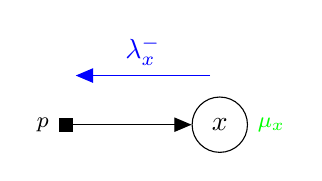
\begin{tikzpicture}
      \centering
      \node[latent, label=right:\textcolor{green}{$\mu_x$}] (x)  {$x$} ;
      \factor[left=1.5 of x] {p} {left:$p$} {} {x} ;

      \node[above=0.5 of x.center] (s1) {} ;
      \node[above=0.5 of p.center] (t1) {};
      \draw[->, blue] (s1) -- (t1) node[midway,above] {$\lambda_x^-$} ;

\end{tikzpicture}

\end{document}
